\documentclass{elsart}

% Use the option doublespacing or reviewcopy to obtain double line spacing
% \documentclass[doublespacing]{elsart}

% if you use PostScript figures in your article
% use the graphics package for simple commands
% \usepackage{graphics}
% or use the graphicx package for more complicated commands
\usepackage{graphicx}
% or use the epsfig package if you prefer to use the old commands
% \usepackage{epsfig}

\usepackage{amssymb,listings}

%% THE ENVIRONMENT \begin{proof} ... \end{proof} PRODUCES AN
%% END-OF-PROOF SIGN.
\newenvironment{proof}{\begin{pf}}{\qed\end{pf}}
%% THE ENVIRONMENT \begin{proof*} ... \end{proof*} SUPPORTS ADDING
%% INFORMATION SUCH AS  'Proof (Sketch)' AS THE LABEL FOR THE PROOF.
\newenvironment{proof*}{\begin{pf*}}{\qed\end{pf*}}

% The lineno packages adds line numbers. Start line numbering with
% \begin{linenumbers}, end it with \end{linenumbers}. Or switch it on
% for the whole article with \linenumbers.
% \usepackage{lineno}
% \linenumbers

\usepackage{listings}
\lstset{mathescape,
        escapechar=\%,
        numbers=left, 
        numberstyle=\tiny, 
        stepnumber=1, 
        numbersep=5pt,
        frame=tb,
        xleftmargin=5mm,
        framexleftmargin=5mm,
        language=Matlab,
        belowcaptionskip=5pt}
\renewcommand{\lstlistingname}{Algorithm}
\usepackage{caption}
\captionsetup[lstlisting]{justification=raggedright}

\newcommand{\hp}{H1$^\prime$}

\begin{document}
\begin{frontmatter}

% Title, authors and addresses

% use the thanksref command within \title, \author or \address for footnotes;
% use the corauthref command within \author for corresponding author footnotes;
% use the ead command for the email address,
% and the form \ead[url] for the home page:
\title{Bucket-Sorted Independent Sets for Algebraic Multigrid}
\author[NREL]{David Alber\corauthref{cor}},
\corauth[cor]{Corresponding author. Address: 1617 Cole Blvd., Mail
  Stop: 1608, Golden, CO 80401}
\ead{david\_alber@nrel.gov}
\ead[url]{http://google.com/ie?q=david+alber+nrel\&num=1}
\author[UIUC]{Luke Olson}
\address[NREL]{Scientific Computing Center\\ National Renewable Energy Laboratory}
\address[UIUC]{Department of Computer Science\\ University of Illinois at Urbana-Champaign}
\ead{lukeo@uiuc.edu}
\ead[url]{http://www.cs.uiuc.edu/homes/lukeo}
% \thanks[label2]{}
% \address{Address\thanksref{label3}}
% \thanks[label3]{}
% use optional labels to link authors explicitly to addresses:
% \author[label1,label2]{}
% \address[label2]{}

\begin{abstract}
\end{abstract}

\begin{keyword}
multigrid \sep parallel algorithms
% keywords here, in the form: keyword \sep keyword

% PACS codes here, in the form: \PACS code \sep code
% \PACS 
\MSC 65F10 \sep 65Y05 \sep 05C69
\end{keyword}
\end{frontmatter}

\section{Introduction}
\label{sec:intro}
The algebraic multigrid (AMG) method~\cite{Ruge1987,Brandt1982} is an
efficient numerical algorithm for finding the solution to numerous
problems, including linear systems $Ax = b$ arising from the
discretization of partial differential equations on structured and
unstructured meshes. In many cases, the computational complexity of
AMG is $O(n)$, where $n$ is the number of unknowns in the linear
system. The linear cost scaling property of AMG makes the method
attractive, especially for large problems.

AMG algorithms are generally divided into two phases: the setup phase
and the solve phase. Setup phase algorithms provide functionality for
constructing elements needed by the solve phase, such as coarse grids,
operators to transfer information between levels of the problem, and
the linear systems to be solved on each level. The solve phase applies
relaxation methods on the problems generated in the setup phase and
uses the transfer operators to move vectors between levels.

In this paper, we focus attention on coarse-grid selection algorithms
in the AMG setup phase. One class of coarse-grid selection algorithms,
independent set-based algorithms, is studied in detail. In
Section~\ref{sec:cgs}, we introduce the coarse-grid selection problems
and the goals of coarse-grid selection algorithms. The components of
independent set-based coarsening algorithms are discussed. 

\section{Coarse-Grid Selection}
\label{sec:cgs}
In AMG, coarse-grid selection is the process of selecting the degrees
of freedom for the coarse level problem. In classical AMG, degrees of
freedom on a coarse level are a subset of the degrees of freedom on a
finer level. Smoothed
aggregation~\cite{Vanek1996,Vanek2001,brezina2005} forms a
coarse-level degree of freedom by aggregating several fine-level
degrees of freedom. In this paper, we study coarsening for classical
AMG.

Given a set of fine-level degrees of freedom, $\Omega_k$, coarse-grid
selection for classical AMG selects a set of coarse-level degrees of
freedom $\Omega_{k+1} \subset \Omega_k$. Several approaches have been
developed for selecting the coarse grid.

Independent set-based algorithms are most numerous and all trace their
roots to the classical AMG coarsening algorithm, RS
coarsening~\cite{Ruge1987}. These methods are our focus and are
discussed in more detail in the next section.

Other methods take substantially different approaches to
coarsening. The coarsening technique in~\cite{Griebel2006} develops a
parallel coarsening algorithm that utilizes RS. On each processor, RS
selects several different coarse grids, and then one coarse grid is
selected per processor in a way to minimize special treatment on
processor boundaries. In~\cite{MacLachlan2006}, a greedy approach is
used to produce a good splitting of the unknowns into fine-grid and
coarse-grid sets. Subdomain blocking techniques~\cite{Krechel2001}
offer another approach for parallel coarse-grid selection by
decoupling coarse grids and alleviating the need for communication on
coarse levels. Compatible relaxation
approaches~\cite{Brandt2000,Livne2004,Brannick2005} form coarse grids
incrementally and decide when the coarse grid is sufficient through a
quality measure based on relaxation.

\subsection{Independent Set-Based Selection}
\label{sec:indep-set-based}
Independent set-based coarse grid selection algorithms implement three
routines to select coarse grids: initialization, independent set
selection, and weight update. A general independent-set based
coarsening algorithm is shown in
Algorithm~\ref{alg:general-indep-set}.
\begin{lstlisting}[caption={Independent Set-Based Coarse Grid
Selection},label=alg:general-indep-set]
%\textsc{Indep-Set-Coarse-Grid-Selection}$(\Omega)$:%
$F \leftarrow \emptyset$
$C \leftarrow \emptyset$
$w \leftarrow\,$%\textsc{Initialize-Weights}$(\Omega)$%
while $\Omega \ne \emptyset$
   $D \leftarrow\,$%\textsc{Select-Indep-Set}$(w,\, \Omega)$%
   $(F,\, C,\, \Omega,\, w) \leftarrow\,$%\textsc{Update-Weights}$(F,\,
                                C,\, \Omega,\, w)$%
end
\end{lstlisting}

Each vertex in the graph is assigned a weight based on its merit to
becoming a $C$-point. The largest weights are conferred to vertices
best suited to become $C$-points. The quality of potential $C$-points
is quantified by \emph{strength of connection} measures. The classical
strength of connection measure is based entirely on the relative sizes
of off-diagonal nonzeros in $A$. In the classical definition, the set
of unknowns that unknown $i$ strongly depends upon is defined as
\begin{equation}
\label{2:eqn:S_i}
S_i = \left\{j: i \ne j \textrm{ and }|a_{ij}| \ge \theta \max_{k \ne
i}|a_{ik}|\right\},
\end{equation}
where $a_{ij}$ is the nonzero in row $i$, column $j$ of matrix $A$ and
$0 < \theta \le 1$. The set of unknowns that $i$ strongly influences,
denoted $S_i^T$, is defined as the set of unknowns that strongly
depend on $i$: $S_i^T = \{j: i \in S_j\}$.

This classical strength definition is formulated based on M-matrix
properties and does not model the influence between unknowns in
general cases. The formulation of new, effective, and inexpensive
strength of connection measures is an active area of
research~\cite{Brannick2005} and has the potential to extend the
applicability of AMG solvers.

Vertex $i$ is eligible to be added to the independent set $D$ if the
following condition is satisfied:
\begin{equation}
  \label{eq:D-selection}
  w_i > w_j,\, \forall j \in S_i \cup S_i^T.
\end{equation}

Many independent set-based coarsening algorithms form $\Omega_{k+1}$
using the following heuristics.
\begin{description}
\item[H1:] For each unknown $j$ that strongly influences $F$-point
  $i$, $j$ is either a $C$-point or strongly depends on a $C$-point
  $k$ that also strongly influences $i$.
\item[H2:] The set of $C$-points needs to form a maximal independent
  set in the reduced graph of $S$ such that no $C$-point strongly
  depends on another $C$-point.
\end{description}
H1 and H2 cannot, in general, be satisfied simultaneously, so H1 is
enforced by independent set-based methods, while H2 serves as a
guideline whose purpose is to encourage selection of small
$|\Omega_{k+1}|$.

Some independent set-based coarsening algorithms use a variant of H1,
called \hp, which is a relaxed version of H1.
\begin{description}
\item[\hp] Each $F$-point must be strongly influenced by at least one
  $C$-point.
\end{description}

\section{Invariance of Selection in Independent Set-Based Methods}
\label{sec:invariance}

Theory is developed in this section to prove coarse-grid selection
invariance in general independent set-based algorithms. The algorithms
considered thus far select independent sets using
(\ref{5:eqn:D-conditions}), meaning $i$ is eligible to be in $D$ if
its weight is larger than the weights of vertices in its neighborhood
$\mathcal{N}_i$. Recall the neighborhood of $i$
(Definition~\ref{3:def:neighborhood}) is the set of vertices strongly
influenced by $i$ or strongly influencing $i$. Algorithms relying on
different and larger neighborhoods, such as \emph{distance-$d$
neighborhoods}, are conceivable.
\begin{defn}
The \emph{distance-$d$ neighborhood} of $i$, denoted
$\mathcal{N}_i^d$, is the set of vertices within $d$ hops of $i$ in
the symmetrized strength matrix, excluding $i$. That is,
$\mathcal{N}_i^d = \left[\bigcup_{j \in
\mathcal{N}_i^{d-1}}\left(\mathcal{N}_j \cup \{j\}\right)\cup
\mathcal{N}_i\right] \setminus \{i\}$, where $d > 0$ and
$\mathcal{N}_i^0 = \emptyset$.
\end{defn}

For a general independent set-based coarse-grid selection algorithm, a
vertex $i$ is eligible to be added to $D$ if
\begin{equation}
\label{5:eqn:general-selection}
w_i > w_j\;\textrm{for all } j \in \mathcal{N}_i^s,
\end{equation}
where $\mathcal{N}_i^s$ is the \emph{selection neighborhood} of
$i$. Although the distance-$d$ neighborhood is a sensible choice for
the selection neighborhood, this discussion is not limited to such
cases. It is assumed, however, the matrix formed by $\mathcal{N}_*^s$
(i.e., the selection sets for all vertices) is symmetric. This is
equivalent to stating if $j \in \mathcal{N}_i^s$, then $i \in
\mathcal{N}_j^s$ for all $i$ and $j$ in the vertex set. Furthermore,
this discussion assumes the weight of vertex $i$ is only decremented
following weight updates and is never modified due to the assignment
of a vertex $j \notin \mathcal{N}_i^s$ to the $C$-point set.

Given a symmetric, but otherwise arbitrary, set of selection
neighborhoods, the set of vertices potentially able to affect the
vertex weight of $i$ or $j \in \mathcal{N}_i^s$ is the \emph{extended
selection neighborhood}.
\begin{defn}
The \emph{extended selection neighborhood} of $i$, denoted
$\mathcal{N}_i^{2s}$, is the union of the selection neighborhood of
$i$ with the selection neighborhoods of the vertices in
$\mathcal{N}_i^s$, excluding $i$. That is, $\mathcal{N}_i^{2s} =
\left[\left(\bigcup_{j \in \mathcal{N}_i^s}\mathcal{N}_j^s\right)\cup
\mathcal{N}_i^s\right] \setminus \{i\}$.
\end{defn}

When a vertex $i$ satisfies the generalized selection
condition~(\ref{5:eqn:general-selection}), no other $C$-point
assignments affect $w_i$. This is formalized below.
\begin{lem}
\label{5:lemma:C-lock}
If (\ref{5:eqn:general-selection}) is satisfied for vertex $i$, then
$i$ must be the next vertex in $\{i\} \cup \mathcal{N}_i^s$ to become
a $C$-point, regardless of any other selections and updates made in
the graph.
\end{lem}
\begin{proof}
The satisfaction of (\ref{5:eqn:general-selection}) means $w_i > w_j$
for all $j \in \mathcal{N}_i^s$. For $i$ to not become a $C$-point,
its weight must become smaller than some $j \in \mathcal{N}_i^s$. The
weight of $i$, however, is not decremented unless some $j \in
\mathcal{N}_i^s$ satisfies~(\ref{5:eqn:general-selection}) and becomes
a $C$-point, which is impossible until after $i$ is assigned to the
$C$-point set.
\end{proof}

To demonstrate all algorithms using the same selection neighborhood
and update rules select identical coarse grids, a proof with an
inductive argument is presented below. The base case is provided by
the first set of vertices satisfying the general selection conditions.
\begin{defn}
Let $D_0$ be the set of all vertices satisfying
(\ref{5:eqn:general-selection}) in the first iteration of coarse-grid
selection.
\end{defn}

Vertices in $D_0$ are destined to become $C$-points regardless of the
algorithm used to build coarse grids. In the independent set-based
algorithms discussed in Chapters~\ref{chap:CGS}
and~\ref{chap:color-based}, all $D_0$ vertices become $C$-points in
the first iteration. Any algorithm constructed, however, eventually
selects all $D_0$ vertices as $C$-points, as proven in the following
lemma.
\begin{lem}
\label{5:lemma:D0_invariant}
Given the same selection neighborhoods and update heuristics, all
algorithms select vertices in $D_0$ as $C$-points.
\end{lem}
\begin{proof}
The proof follows from Lemma~\ref{5:lemma:C-lock}. All vertices in
$D_0$ satisfy the selection condition~(\ref{5:eqn:general-selection}),
so the assignment of any other $C$-point has no effect on the weight
of a $D_0$ vertex.
\end{proof}

Lemma~\ref{5:lemma:D0_invariant} states that any coarse-grid selection
method using the general selection condition invariably selects $D_0$
vertices as $C$-points. This result is used in the proof of the next
theorem.

\begin{thm}
\label{5:theorem:invariance}
All independent set-based coarse-grid selection algorithms given the
same initial weights and using the same selection neighborhood,
selection criterion based on~(\ref{5:eqn:general-selection}), and
weight update heuristics as described above select identical coarse
grids.
\end{thm}
\begin{proof}
Let $c$ be the vertices in $\mathcal{N}_i^{2s}$ satisfying the
conditions for $D$ in some arbitrary iteration. Suppose assigning
vertices $c_1 \subset c$ to the $C$-point set leads to $w_i > w_j$ for
all $j \in \mathcal{N}_i^s$. Also suppose assigning $c_2 \subset c$,
$c_1 \ne c_2$, to the $C$-point set leads to the existence of some $j
\in \mathcal{N}_i^s$ such that $w_j > w_k$ for all $k \in
\mathcal{N}_j^s$.

For both conditions to be true, one or both of the following cases
must be satisfied.
\begin{enumerate}
\item The value of $w_i$ is smaller when $c_2$ is added to the
  $C$-point set than when $c_1$ is added. For this case, it must be
  true that $|c_2 \cap \mathcal{N}_i^s| > |c_1 \cap \mathcal{N}_i^s|$.
\item The value of $w_j$ is larger when $c_2$ is added to the
  $C$-point set than when $c_1$ is added. For this case, it must be
  true that $|c_2 \cap \mathcal{N}_j^s| < |c_1 \cap
  \mathcal{N}_j^s|$.
\end{enumerate}

Case~1 creates a contradiction. If $|c_2 \cap \mathcal{N}_i^s| > |c_1
\cap \mathcal{N}_i^s|$, then $(c \setminus c_1) \cap \mathcal{N}_i^s
\ne \emptyset$. Following the assignment of the vertices in $c_1$ to
the $C$-point set, there remains some $k \in \mathcal{N}_i^s$ that is
also in $c$. Therefore, $w_k > w_i$, contradicting the first assumed
condition.

Case~2 is similarly impossible. If $|c_2 \cap \mathcal{N}_j^s| < |c_1
\cap \mathcal{N}_j^s|$, then $(c \setminus c_2) \cap \mathcal{N}_j^s
\ne \emptyset$. Following the assignment of the vertices in $c_2$ to
the $C$-point set, there remains some $k \in \mathcal{N}_j^s$ that is
also in $c$. Therefore, $w_k > w_j$, contradicting the second assumed
condition.

Both cases are impossible, so the order of $C$-point selection within
the selection neighborhood of each vertex is invariant. Combined with
Lemma~\ref{5:lemma:D0_invariant} as the base case, this proves by
induction the invariance of coarse-grid selection for all algorithms
using identical selection conditions.
\end{proof}

\begin{rem}
CLJP and CLJP-c use the distance-one neighborhood as the selection
neighborhood, (\ref{5:eqn:D-conditions}) as the selection criterion,
and the weight update heuristics in
Algorithm~\ref{3:alg:CLJP-update-heuristics}. Given the same initial
weights, all algorithms based on the parameters utilized by CLJP and
CLJP-c select identical coarse grids.
\end{rem}

Theorem~\ref{5:theorem:invariance} is an important result about the
nature of coarse grids selected by general independent set-based
algorithms. This information enables the design and implementation of
new algorithms that yield identical coarse grids using different and
possibly more efficient techniques.

\section{Bucket Sorted Independent Set Selection}
\label{5:sec:contribution}

\subsection{CLJP-c}
Recall that CLJP-c colors the graph of $S$ before selecting
$C$-points, and the colors are used as one component of the vertex
weights. As a result, the structure of the coarse grids selected is
improved. More formally, the use of graph coloring provides the
following important result.
\begin{thm}
\label{5:theorem:CLJPc-neighbor-independence}
For all pairs of vertices $i$ and $j \in \mathcal{N}_i$ CLJP-c
guarantees $w_i \ne w_j$.
\end{thm}
\begin{proof}
Assume two adjacent vertices $i$ and $j$ have the same weight. That is,
$|S_i^T| = |S_j^T|$ and the weight augmentation provided through
coloring is the same for $i$ and $j$. The graph of $S$, however, is
colored such that $i$ and $j$ are different colors for all $j \in
\mathcal{N}_i$, so a contradiction is reached.
\end{proof}
Theorem~\ref{5:theorem:CLJPc-neighbor-independence} establishes that
all adjacent vertices have different weights in CLJP-c, which is not
guaranteed in CLJP, although is unlikely to occur. The following
corollaries are a result of
Theorem~\ref{5:theorem:CLJPc-neighbor-independence}.
\begin{cor}
Any set of vertices in the graph of $S$ that share the same weight is
an independent set.
\end{cor}
\begin{cor}
\label{5:cor:max-weight-indep-set}
The set of vertices with the largest weight in the graph of $S$ form
an independent set satisfying~\ref{5:eqn:D-conditions}. That is, each
vertex in that independent set has a uniquely maximal weight in its
neighborhood.
\end{cor}
The first corollary states that independent sets can be selected in
the graph simply by selecting sets of vertices with the same
weight. Corollary~\ref{5:cor:max-weight-indep-set} refines this
observation to a subset of vertices guaranteed to satisfy the
selection criterion. In particular, it shows it is possible to build
the coarse grid by selecting vertices with the maximum weight,
updating weights, selecting the next set of vertices with maximum
weight, and so on. This approach is taken by the algorithm developed
in Section~\ref{5:sec:contribution}. It is proven in
Section~\ref{5:sec:cg-invariance} that despite the difference in
approach, the resulting coarse grid is the same as that selected by
CLJP-c.

\subsection{BSIS}
\label{sec:bsis}
In this section, new techniques for searching the graph of $S$ for new
$C$-points and subsequently updating the weights of remaining vertices
are developed. The new algorithm is labeled Bucket Sorted Independent
Sets (BSIS) to reflect the data structure used.

Like CLJP-c, BSIS depends on graph coloring, but utilizes modified
routines for search and weight update. Furthermore, rather than
applying the color information to augment vertex weights, BSIS uses
the colors in a bucket data structure. Once initialized, this data
structure selects independent sets, which satisfy the conditions in
(\ref{5:eqn:D-conditions}), in constant time.

\subsection{Motivation}
\label{sec:motivation}
CLJP and its descendents select an independent set $D$ in each
iteration. Stated originally in Section~\ref{3:sec:CLJP}, the
condition for selecting $D$ is that all vertices $i \in D$ must
satisfy
\begin{equation}
\label{5:eqn:D-conditions}
w_i > w_j\;\textrm{for all } j \in \mathcal{N}_i.
\end{equation}
CLJP and CLJP-c rely on a search routine to locate locally maximal
weights and on a weight update routine to modify weights of vertices
connected to new $C$-points.

The algorithms for searching and updating vertex weights in CLJP in
detail are examined in this section. In particular, the impact of
using a sparse matrix format on the coarsening procedure. The
pseudo-code below assumes the software uses a compressed sparse row
(CSR)~\cite{saadBook} matrix format or other similar format, which are
common matrix formats in numerical software. CSR provides low memory
costs for storing sparse matrices and provides efficient access to the
nonzeros in a row. Accessing the nonzeros in a column is an expensive
operation in this format and strongly influences the weight update
routine in CLJP-style algorithms because $S$ is, in general, not
symmetric.

The search step in CLJP is implemented as shown in
Algorithm~\ref{5:alg:search}.
\begin{lstlisting}[caption={Coarse-Grid Selection Graph Search},label=5:alg:search]
%\textsc{Search-Graph}$(S,\, C,\, F)$%
$D \leftarrow \emptyset$
for $i$ in $(C \cup F)$
  if $w_i > w_j,\,\forall j \in \mathcal{N}_i$
    $D \leftarrow D \cup \{i\}$
  end
end
return $D$
\end{lstlisting}
% \begin{algorithm}[h]
% \caption{Coarse-Grid Selection Graph Search}
% \label{5:alg:search}
% \textsc{Search-Graph}$(S,\, C,\, F)$ \{
% \begin{algorithmic}[1]
% \STATE $D \leftarrow \emptyset$
% \FORALL{$i \notin (C \cup F)$}
% \IF{$w_i > w_j,\,\forall j \in \mathcal{N}_i$}
% \STATE $D \leftarrow D \cup \{i\}$
% \ENDIF
% \ENDFOR
% \RETURN $D$
% \end{algorithmic}
% \}
% \end{algorithm}
In the first iteration, Line~3 is run $2|E|$ times. The total cost of
search in constructing the coarse grid depends on the number of
iterations needed. Even in the best case of $\Omega(E)$ time, the cost
is significant when the graph contains large numbers of edges, as
usually happens on the lower levels in the grid hierarchy
(see~\cite{alber-PCGS} for examples). In the next section, a new
technique is introduced for conducting the search in coarse-grid
selection algorithms independent of the number of edges in the graph.

Pseudo-code for the weight update in CLJP is shown in Algorithm~\ref{5:alg:setup}.
\begin{lstlisting}[caption={CLJP Weight Update for CSR Matrix},label=5:alg:setup]
%\textsc{Update-Weights}$(S,\, D,\, C,\, F,\, w)$%
for $d \in D$
  for $i \in S_d$
    $w_i \leftarrow w_i - 1$    //see %Figure~\ref{3:fig:CLJP-update-heuristics} left%
    $S_d = S_d \setminus \{i\}$ //removing edge from graph
  end
end
for $i \notin (C \cup F)$
  for $k$ originally in $S_i$
    if $k \in D$
      mark $k$ NEW-C-POINT
    end
  end
  for $j \in S_i$
    if $j \notin D$
      for $k \in S_j$
        if $k$ is marked NEW-C-POINT      // $i$ and $j$ mutually influenced by $k$
          $w_j \leftarrow w_j - 1$        // see %Figure~\ref{3:fig:CLJP-update-heuristics} right%
          $S_i = S_i \setminus \{j\}$     // remove edge from $j$ to $i$
        end
      end
    end
  end
  for $k$ originally in $S_i$
    if $k \in D$
      unmark $k$
      $S_i = S_i \setminus \{k\}$         // remove edge from $k$ to $i$, if present
    end
  end
end
\end{lstlisting}
%\begin{algorithm}[h]
%\caption{CLJP Weight Update for CSR Matrix}
%\label{5:alg:setup}
%\textsc{Update-Weights}$(S,\, D,\, C,\, F,\, w)$ \{
%\begin{algorithmic}[1]
%\FORALL{$d \in D$}
%\FORALL{$i \in S_d$}
%\STATE $w_i \leftarrow w_i - 1$ \COMMENT{see
%  Figure~\ref{3:fig:CLJP-update-heuristics} left}
%\STATE $S_d = S_d \setminus \{i\}$ \COMMENT{removing edge from graph}
%\ENDFOR
%\ENDFOR
%\FORALL{$i \notin (C \cup F)$}
%\FORALL{$k$ originally in $S_i$}
%\IF{$k \in D$}
%\STATE mark $k$ NEW-C-POINT
%\ENDIF
%\ENDFOR
%\FORALL{$j \in S_i$}
%\IF{$j \notin D$}
%\FORALL{$k \in S_j$}
%\IF[$i$ and $j$ mutually influenced by $k$]{$k$ is marked NEW-C-POINT}
%\STATE $w_j \leftarrow w_j - 1$ \COMMENT{see
%  Figure~\ref{3:fig:CLJP-update-heuristics} right}
%\STATE $S_i = S_i \setminus \{j\}$ \COMMENT{remove edge from $j$ to $i$}
%\ENDIF
%\ENDFOR
%\ENDIF
%\ENDFOR
%\FORALL{$k$ originally in $S_i$}
%\IF{$k \in D$}
%\STATE unmark $k$
%\STATE $S_i = S_i \setminus \{k\}$ \COMMENT{remove edge from $k$ to $i$,
%  if present}
%\ENDIF
%\ENDFOR
%\ENDFOR
%\end{algorithmic}
%\}
%\end{algorithm}
The level of complication in this update routine is due to the CSR
format and the need to find vertices strongly influenced by new
$C$-points. When a new $C$-point $k$ is selected, the first type of
weight update is trivial since determining the vertices in $S_k$ is
inexpensive. The second type of update is more expensive since the
vertices influenced by $k$ are difficult to determine in a CSR
format. The update requires a search of many vertices $i$ and all of
their strong influencing neighbors $j$. The routine then searches
strongly influencing $j$ to determine if any $k \in D$ strongly
influences both $i$ and $j$. The cost increases dramatically as the
density of $S$ increases. Large operator complexities have a
disproportionately large impact on coarse-grid selection run time. In
the next section, a modified update routine to compliment the new
search technique is introduced.

\subsection{Bucket Sorted Independent Sets Algorithm}
The BSIS algorithm creates a bucket data structure enabling a search
for new $C$-points without individually scanning each vertex and
associated edges. Figure~\ref{5:fig:bucket-algorithm} illustrates the
bucket data structure. The number of buckets in the data structure is
$\max_{i \in S}|S_i^T|$ times the number of colors in the graph. That
is, each possible weight in $S$ has its own bucket. The vertices are
distributed to the appropriate buckets during the setup of the
coarse-grid selection algorithm, where the bucket of a newly placed
vertex depends on the number of vertices it strongly influences and
its color. For example, Vertex~14 strongly influences six vertices and
is black. Therefore, it is placed into the black bucket in the sixth
group of buckets. More notably, the vertices in a bucket form an
independent set (e.g., vertices 4, 16, and 21).

In each iteration, the non-empty bucket with largest weight forms $D$
(see Corollary~\ref{5:cor:max-weight-indep-set}). These vertices are
assigned to the $C$-point set and removed from the data
structure. Vertex weight updates lead to corresponding updates to the
data structure, and new $F$-points are removed from the data
structure. These operations continue until all buckets are empty, at
which point the coarse-grid selection is
complete. Algorithms~\ref{5:alg:BSIS-setup},
\ref{5:alg:BSIS-indep-set-select}, and~\ref{5:alg:BSIS-weight-update}
outline the operations discussed above.
\begin{lstlisting}[caption={BSIS Data Structure Setup},label=5:alg:BSIS-setup]
%\textsc{BSIS-Setup}$(S)$%
for $i \in V$
  $bucketID \leftarrow (w_i-1)\cdot numColors + color_i$
  $bucket[bucketID].\textsc{Insert}(i)$
end
\end{lstlisting}
% \begin{algorithm}[!h]
% \caption{BSIS Data Structure Setup}
% \label{5:alg:BSIS-setup}
% \textsc{BSIS-Setup}$(S)$ \{
% \begin{algorithmic}[1]
% \FORALL{$i \in V$}
% \STATE $bucketID \leftarrow (w_i-1)\cdot numColors + color_i$
% \STATE $bucket[bucketID].\textsc{Insert}(i)$
% \ENDFOR
% \end{algorithmic}
% \}
% \end{algorithm}
\begin{lstlisting}[caption={Independent Set Selection},label=5:alg:BSIS-indep-set-select]
%\textsc{BSIS-Independent-Set-Selection}$(S)$%
return non-empty $bucket$ with largest $bucketID$
\end{lstlisting}
% \begin{algorithm}[!h]
% \caption{Independent Set Selection}
% \label{5:alg:BSIS-indep-set-select}
% \textsc{BSIS-Independent-Set-Selection}$(S)$ \{
% \begin{algorithmic}[1]
% \RETURN non-empty $bucket$ with largest $bucketID$
% \end{algorithmic}
% \}
% \end{algorithm}
\begin{lstlisting}[caption={BSIS Weight Update},label=5:alg:BSIS-weight-update]
%\textsc{BSIS-Weight-Update}$(S)$%
$bucketID \leftarrow (w_i-1)\cdot numColors + color_i$
$bucket[bucketID].\textsc{Remove}(i)$
$bucket[bucketID - numColors].\textsc{Insert}(i)$
\end{lstlisting}
%\begin{algorithm}[!h]
%\caption{BSIS Weight Update}
%\label{5:alg:BSIS-weight-update}
%\textsc{BSIS-Weight-Update}$(S)$ \{
%\begin{algorithmic}[1]
%\STATE $bucketID \leftarrow (w_i-1)\cdot numColors + color_i$
%\STATE $bucket[bucketID].\textsc{Remove}(i)$
%\STATE $bucket[bucketID - numColors].\textsc{Insert}(i)$
%\end{algorithmic}
%\}
%\end{algorithm}
\begin{figure}
  \begin{center}
    %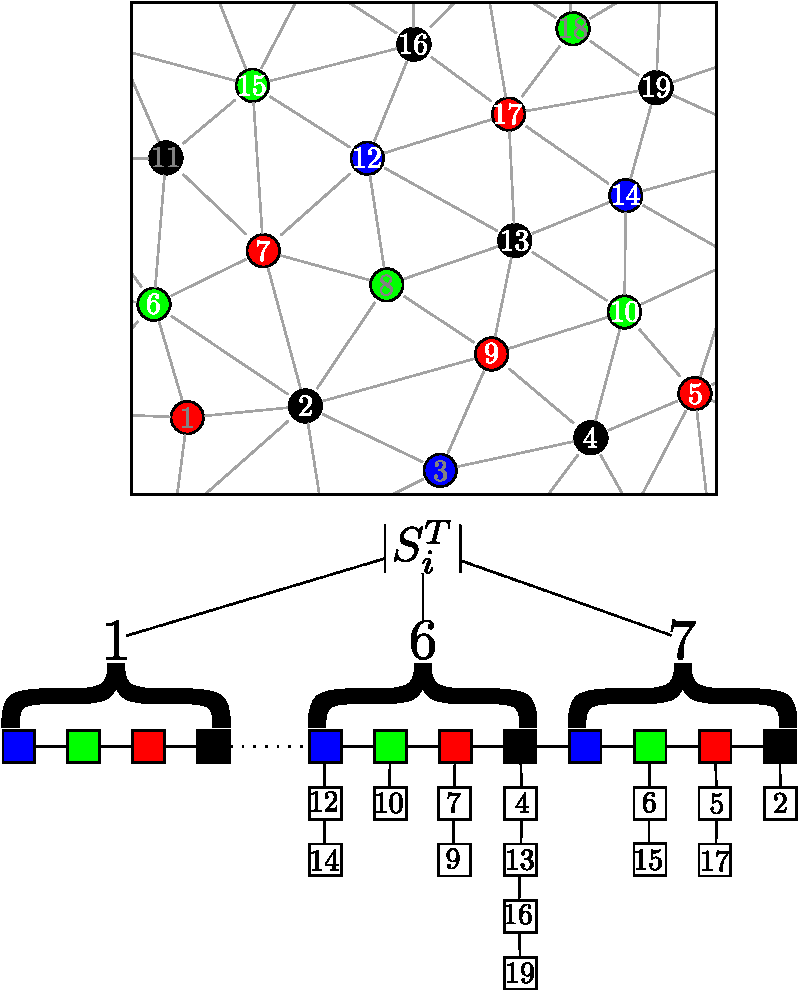
\includegraphics[width=0.8\textwidth]{images/bucket-algorithm}
    \includegraphics[width=0.98\textwidth]{images/BSIS/initial}
    \caption{The BSIS data structure.}
    \label{5:fig:bucket-algorithm}
  \end{center}
\end{figure}

Figure~\ref{5:fig:bucket-algorithm-cp1} illustrates the graph and data
structure following the first iteration of the algorithm. Vertex~10
has become a $C$-point and its neighbors weights have been
updated. Vertices assigned to $F$ or $C$ are removed from the data
structure and other affected vertices are moved to new locations in
the data structure. Such vertices are highlighted in red.
\begin{figure}
  \begin{center}
    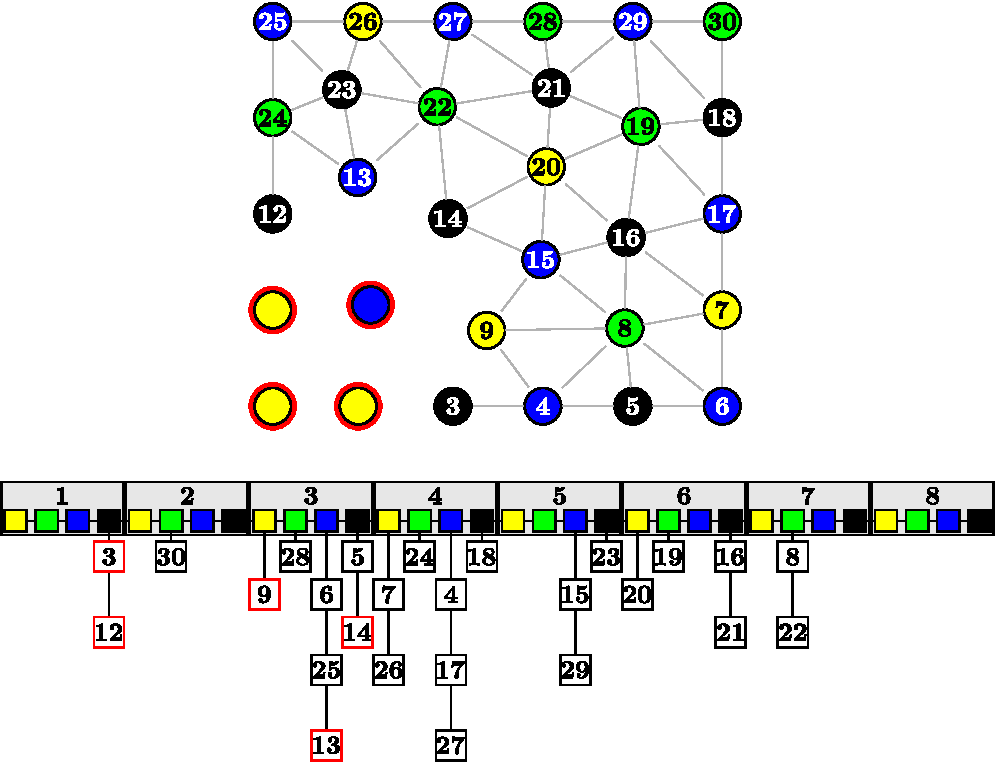
\includegraphics[width=0.98\textwidth]{images/BSIS/cp1}
    \caption{The BSIS data structure after selecting the first
    $C$-point (Vertex 10). The weights of neighbors of the new
    $C$-point are updated. Some neighbors become $F$-points and are
    removed from the data structure. Vertices removed from the data
    structure are highlighted with a red ring in the graph, while
    other neighbors are moved to new locations in the data structure
    and are highlighted (to help in reading the figure) in the data
    structure with a red box.}
    \label{5:fig:bucket-algorithm-cp1}
  \end{center}
\end{figure}

The weight update routine described in
Section~\ref{5:sec:s-and-w-update} is very expensive in this context
because some iterations of BSIS select few $C$-points. For a graph
with a large number of colors, BSIS may execute dozens or hundreds of
low-cost iterations to select a coarse grid. Recall the weight update
routine described loops through all unassigned vertices each time it
is called, so when it is run by BSIS, work is done on many unaffected
vertices, which is computationally inefficient.

The largest factor in the cost of the weight update results from
searching for the second type of weight update in
Algorithm~\ref{5:alg:setup}, which is done by looping through all
unassigned vertices since a new $C$-point cannot easily determine
which vertices it strongly influences in a CSR matrix. It is less
expensive in this situation to construct the transpose of $S$ than to
search the entire graph in each iteration. In $S^T$, a $C$-point
quickly determines which vertices it influences and ``paints''
them. The algorithm then loops through all painted vertices and
determines if any are neighbors. This is a simple solution that has a
dramatic effect on the performance of BSIS, although the update cost
remains approximately equivalent to the cost in
CLJP-c. Chapter~\ref{chap:conclusions} describes plans for continued
investigation into decreasing the cost of weight update in coarsening
algorithms.

\subsection{Weight Update Aggregation}
\label{5:sec:agg}
Whenever a vertex weight is updated, BSIS moves the corresponding
vertex to a new location in the data structure. During the selection
of the coarse grid, the cost of the updates to the data structure is
non-trivial and, as shown in this section, unnecessary.

Only one bucket in the data is touched during the $C$-point selection
step: the largest weight non-empty bucket in the data structure. Other
buckets are subsequently affected by the weight updates resulting from
new $C$-point assignments. A different approach is possible, however,
since the only bucket that must contain the correct vertices is the
one from which $C$-points are selected.

To save cost, we suggest a lazy approach based on aggregating the cost
of the updating vertex weights. Rather than investing computation into
maintaining accuracy in the data structure, a less expensive mechanism
to test if a vertex is in the correct location is provided. When a
weight is updated, the vertex is not moved until it is found in the
bucket being used as the new independent set $D$.

Figure~\ref{5:fig:cp1-agg} depicts the data structure after the first
set of $C$-points is selected.
\begin{figure}
  \begin{center}
    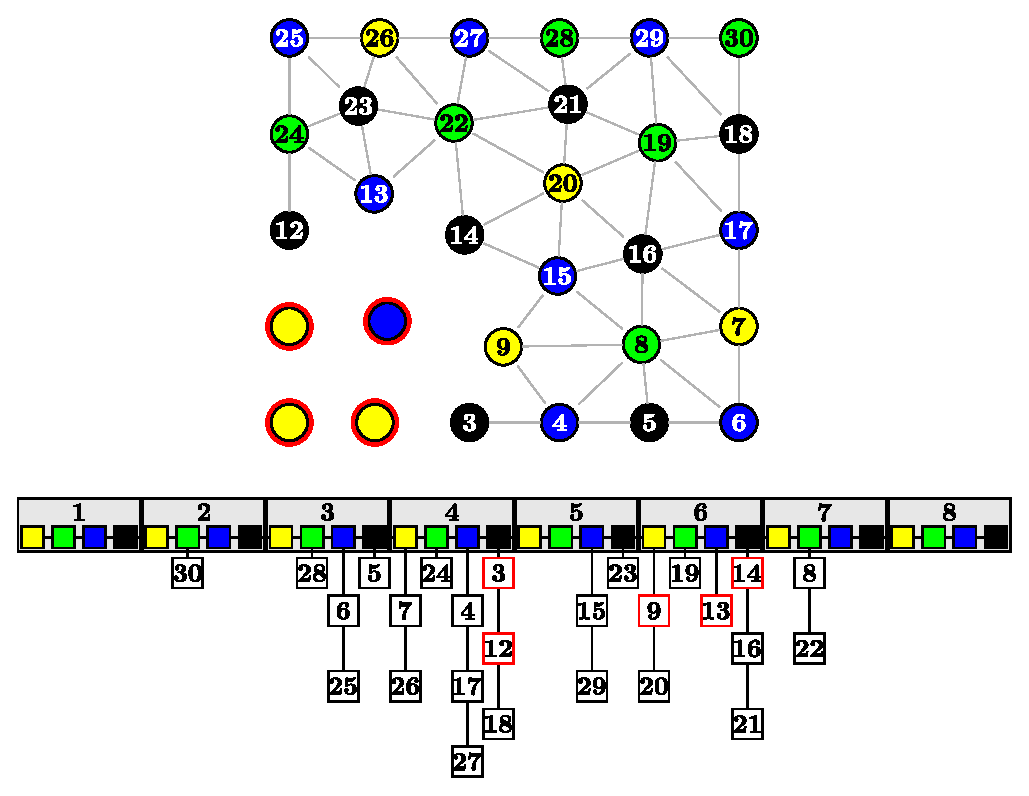
\includegraphics[width=0.98\textwidth]{images/BSIS/cp1-agg}
    \caption{The BSIS data structure after selecting the first
    $C$-point (Vertex 10) with aggregate weight updates.}
    \label{5:fig:cp1-agg}
  \end{center}
\end{figure}
Rather than moving vertices to new buckets, the method now keeps them
in the same location and only moves them when necessary. As shown in
Section~\ref{5:sec:experiments}, aggregation of the weight updates
leads to significant savings in computational cost.

\subsection{Experimental Results}
\label{5:sec:experiments}
To demonstrate BSIS, the algorithm is compared with CLJP-c. The test
problem is the 3D 7-point Laplacian on a structured grid:
\begin{eqnarray}
\label{5:eqn:Lap} -\Delta u & = & 0 \quad \textrm{on } \Omega \qquad
(\Omega = (0, 1)^3),\\
\nonumber u & = & 0 \quad \textrm{on } \partial \Omega.
\end{eqnarray}
A 7-point Laplacian is selected since it is a common initial test
problem and structured problems often lead to the largest operator
complexities for coarsening algorithms satisfying heuristic H1. By
creating larger operator complexities, the algorithms are forced to
traverse more edges in the graph, leading to more work.

Timing data for the selection of all coarse grids in the hierarchy is
reported. This time includes the cost for all parts of the algorithms,
including the graph coloring phase. AMG solve phase information is not
reported since the algorithms produce identical coarse grids and since
information on solve phase performance for AMG with CLJP-c is
documented in~\cite{alber-cljpc,alber-PCGS}.

The smallest problem is a $30 \times 30 \times 30$ grid. Subsequent
problems are grids of size $60^3$, $90^3$, up to $210^3$. The largest
problem is 343 times larger than the smallest problem and contains
more than nine million degrees of freedom.

Results for the experiment are presented in
Figure~\ref{5:fig:results-full}.
\begin{figure}
  \begin{center}
    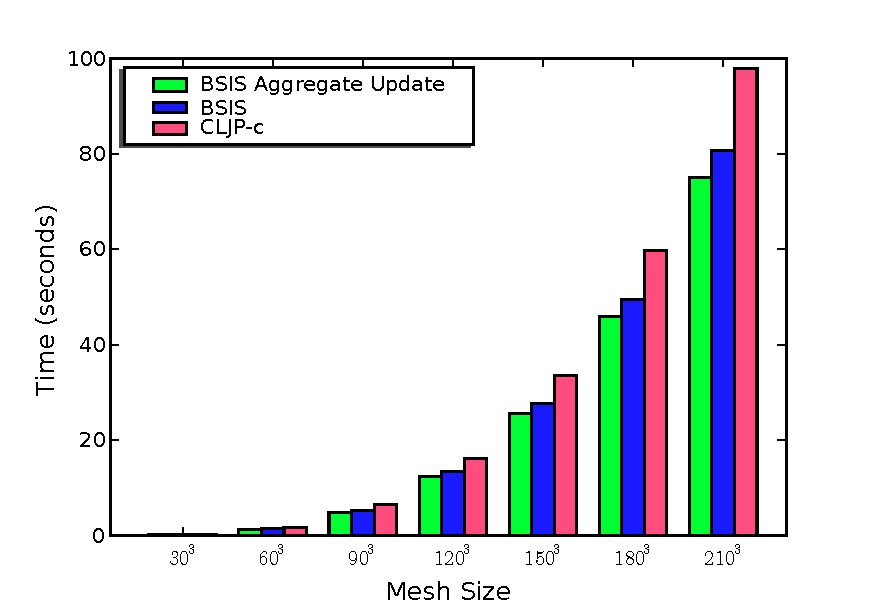
\includegraphics[width=0.75\textwidth]{images/agg-no-scaling}
    \caption{Coarse-grid selection times using BSIS with aggregate
    weight update, standard BSIS, and CLJP-c on the 7-point
    Laplacian.}
    \label{5:fig:results-full}
  \end{center}
\end{figure}
BSIS completes coarse-grid construction in less time than CLJP-c in
every case, and BSIS with aggregate weight update performs
significantly better than standard BSIS. For the largest problems BSIS
is approximately 17\% cheaper than CLJP-c. BSIS with aggregate weight
updates is 23\% cheaper on the largest problems. The benefit is
magnified, relative to CLJP-c, for the smaller problems.

Experiment (\ref{5:eqn:Lap}) demonstrates the effectiveness and
competitiveness of the bucket technique. Increased efficiency for the
BSIS algorithm is anticipated through further research. Furthermore,
the methods and concepts in this research are also applicable to other
coarsening algorithms and possibly to other elements in the AMG setup
phase.

\subsection{BSIS Variants}
The ideas developed in this chapter are applicable to other coarsening
algorithms that utilize a graph coloring step, such as color-based
methods designed to satisfy heuristic H1$^\prime$. The PMIS-c1
algorithm is expected to benefit from BSIS and is expected to perform
naturally in parallel since vertex weights are not updated in PMIS.

\subsection{Parallelizing BSIS}
Using BSIS in a parallel algorithm presents challenges because the
parallelism in BSIS is very fine-grained. Its elegance and potential
to greatly improve the efficiency of coarse-grid selection motivates
the development of parallel algorithms incorporating BSIS. Several
alternatives are explored in this section.

The first idea is called the boundary painting method and takes
advantage of the invariance between coarse grids selected by BSIS and
CLJP-c. The idea is to use BSIS to select as many of the interior
$C$-points as possible before doing any communication with neighboring
processors. All vertices belonging to a processor are colored and
inserted into the BSIS data structure. The processor boundary
vertices, however, are ``painted''. If a painted vertex is in a set
$D$ in some iteration, then the vertex is not added to $C$. It is
instead removed from the data structure and its on-processor neighbors
are also painted. Figure~\ref{5:fig:cp1-parallel} illustrates the
first iteration of the painted boundary method with weight update
aggregation. The data structure shown is for the left domain.
\begin{figure}
  \begin{center}
    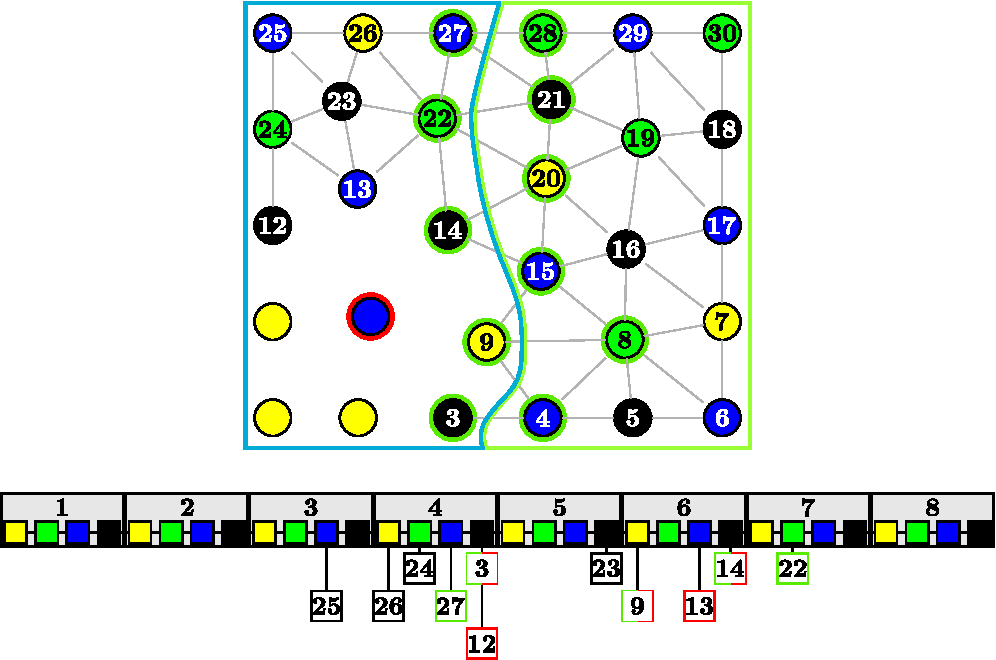
\includegraphics[width=0.98\textwidth]{images/BSIS/cp1p}
    \caption{The painted boundary method with aggregate weight
    updates following one iteration. The data structure is for the
    left domain. Painted vertices are marked with a green ring in the
    graph and a green box in the data structure. Vertices in the data
    structure that are half green and half red are painted and also
    have had their weights updated.}
    \label{5:fig:cp1-parallel}
  \end{center}
\end{figure}
The first iteration selects a new $C$-point, but does not select any
painted vertices. In the second iteration, Vertex~22 is selected, but
is already painted. Therefore, on-processor neighbors of Vertex~22 are
also painted (see Figure~\ref{5:fig:cp2-parallel}).
\begin{figure}
  \begin{center}
    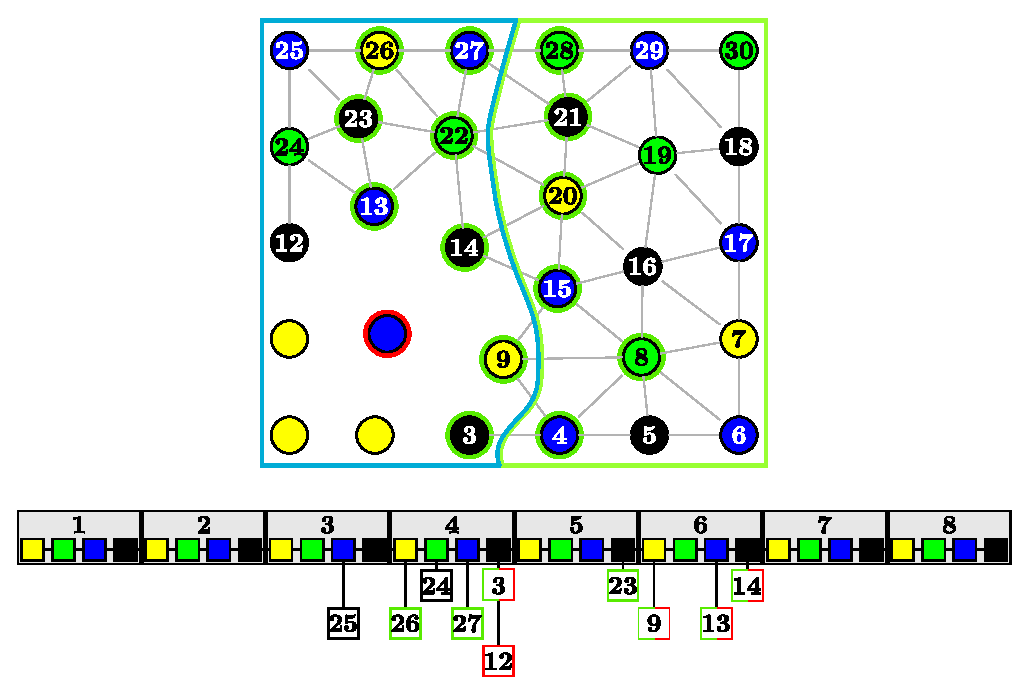
\includegraphics[width=0.98\textwidth]{images/BSIS/cp2p}
    \caption{The painted boundary method with aggregate weight
    updates following the second iteration. In this iteration a
    painted vertex was selected, leading to the painting of its
    on-processor neighbors.}
    \label{5:fig:cp2-parallel}
  \end{center}
\end{figure}
The method finishes when the data structure is emptied of all
vertices. The product is now three disjoint sets: $C$ and $F$, as
usual, but also a set of painted vertices. The painted vertices are
the vertices that cannot be assigned to the $F$ or $C$ set without
communication with another processor. The information is provided to
CLJP-c, which handles the parallel portion of the algorithm.

The painted boundary approach is ideal given large numbers of interior
vertices, which can be guaranteed on most problems for the fine grid.
A side-effect of H1-based coarsening algorithms, however, is the
creation of denser graphs on coarse levels. One solution is to use the
painted boundary method on fine levels and then switch to CLJP-c
further along in the coarsening process. The issue is a smaller
concern for H1$^\prime$-based coarsening using BSIS since these
methods produce small operator complexities that do not grow as the
size of the problem is increased. In all cases, however, the number of
processor boundary vertices relative to the number of interior
vertices increases as the number of unknowns per processor decreases
(e.g., on coarse levels). A few techniques may be applicable in this
situation. The easiest solution is to simply use CLJP-c, or some other
coarsening algorithm, on the coarser levels where few vertices are
found. Although BSIS does not decrease in cost at this point, the
total cost on the levels when BSIS is not used is low due to low
complexity of coarse grids. A second approach is the application of a
dynamic load balancing algorithm to increase the number of vertices on
a processor (and, thus, decrease communication costs). If the number
of vertices per processor per level is maintained at a high enough
level, BSIS is still valuable on coarse grids. A third option is to
replicate the operator matrix on processors, which leads to processors
doing more of the same work, but by avoiding communication. The second
and third ideas are similar in nature and both involve using dynamic
load balancing
techniques~\cite{DevineBomanKarypisPP04,CybDLB,deCoughnyLB,SchloegelLB,ZoltanParHyp06ipdps,ZoltanParHypRepart07}.

\section{Conclusions}
\label{sec:conclusions}


\bibliographystyle{elsart-num}
\bibliography{paper}

\end{document}
